%!TEX root = ../main.tex
\chapter{Justificación técnica y diseño de la solución}\label{cap:marco-tecnologico}

\section{Arquitectura de la solución}

La solución propuesta se organiza mediante una arquitectura modular de integración, diseñada para automatizar la comunicación entre los sistemas internos involucrados en el proceso de facturación y las entidades bancarias responsables de procesar el financiamiento y desembolso de las unidades facturadas.

La arquitectura contempla la convivencia de aplicaciones existentes y componentes desarrollados con tecnologías más actuales. Esta decisión permite mantener la continuidad operativa de los procesos utilizados por los usuarios, evitando reemplazar de forma inmediata el sistema legado, y al mismo tiempo incorporar capacidades modernas para el consumo y exposición de servicios web.

La solución se compone principalmente de las aplicaciones VH Legacy, SAI y VH Connect. VH Legacy es la aplicación utilizada por los usuarios para consultar información de crédito y gestionar operaciones de facturación. SAI participa como intermediario en el flujo de facturación y comunica a VH Connect la información de las facturas que alcanzaron el estado de legalidad. Por su parte, VH Connect centraliza la lógica de integración bancaria, recibe la información enviada por SAI, la almacena y prepara las solicitudes requeridas por las entidades financieras, procesando además las respuestas devueltas por dichas entidades.

La comunicación entre estos componentes combina servicios síncronos, para la recepción de legalidades desde SAI, con integraciones REST hacia las entidades bancarias, cuya estructura varía según el país. El detalle de cada integración, así como las particularidades entre Chile y Perú, se desarrolla en las secciones de Componentes principales y Flujos principales de la solución.

La base de datos Oracle, compartida entre VH Legacy y VH Connect, concentra la información operativa necesaria para la facturación, el crédito disponible y los indicadores que permiten identificar el estado de reporte de cada operación ante las entidades bancarias. Ante errores técnicos, rechazos o fallas de comunicación, la solución cuenta con mecanismos de notificación y reintento que se describen más adelante.

En conjunto, la arquitectura permite separar las responsabilidades de cada sistema, conservar las aplicaciones existentes y centralizar la integración bancaria en VH Connect. De esta forma, se facilita el mantenimiento, se mejora la trazabilidad de las operaciones y se establece una base que puede extenderse en el futuro para incorporar nuevas entidades bancarias, países o aplicaciones internas.

Es importante delimitar qué elementos de esta arquitectura corresponden a infraestructura y funcionalidad ya existente en la organización, y cuáles constituyen la propuesta desarrollada en el marco de este trabajo. VH Legacy, SAI y VH Connect son aplicaciones que ya existen y conviven en producción: VH Connect ya recibe y persiste la información de legalidad de facturas enviada por SAI, las pantallas CR08 y CR12 ya permiten consultar el crédito disponible de cada concesionario, y la pantalla DU13 ya genera el pedido de facturación. De igual manera, las tablas 010\_CLIENTES, 002\_UNIDADES, 222\_MODELOS y 042\_ALTORDEN ya forman parte de la base de datos Oracle compartida.

Sin embargo, ninguno de estos componentes cuenta actualmente con comunicación automatizada con las entidades bancarias. Hoy, la actualización del crédito disponible es un proceso manual: el usuario de cuentas a cobrar debe consultar el home banking de cada entidad bancaria y cargar posteriormente cada valor a mano en la casa matriz correspondiente. De manera análoga, el reporte de facturas hacia los bancos no cuenta con una integración que confirme el resultado de cada envío: en Chile se realiza mediante un archivo transferido por FTP, cuyo envío dispara el usuario, y en Perú mediante una planilla de Excel armada manualmente. La propuesta desarrollada en este trabajo consiste, precisamente, en incorporar dicha comunicación bancaria: la autenticación y consulta/actualización de crédito desde VH Legacy, el informe automatizado de facturas desde VH Connect, las columnas REPORTED\_FORUM y REPORTED\_SANTANDER y las tablas 055\_TRANSACCIONES\_CREDITO y 040\_LOTES\_FACT en la base de datos, la unificación de las pantallas CR08 y CR12, y la incorporación de la pantalla Alta Dua File para el caso particular de Perú. Estos elementos se describen en las secciones siguientes en términos de diseño propuesto, aun cuando se emplee tiempo presente por convención descriptiva habitual en este tipo de documentos.

\subsection{Componentes principales}

\subsubsection{VH Legacy}

VH Legacy es la aplicación legada desarrollada en Java 6, cuya interfaz de usuario fue implementada mediante JavaServer Faces. Es utilizada por los usuarios operativos para consultar el crédito disponible y gestionar operaciones vinculadas con la facturación de unidades financiadas.

Desde VH Legacy, el usuario puede solicitar la actualización del crédito disponible ante la entidad bancaria correspondiente. Esta consulta se realiza mediante servicios REST y los resultados se reflejan en la base de datos Oracle, permitiendo que la información esté disponible antes de continuar con una operación de facturación.

En Chile, el crédito se administra a nivel de la casa matriz del concesionario, aun cuando este posea sucursales. En Perú, la operación se realiza únicamente a nivel de casas matrices. Para Chile se contempla, además de la consulta manual, la implementación de un proceso programado de actualización horaria. En Perú, la actualización se mantiene como una acción manual que el usuario puede ejecutar cuando lo requiera.

\subsubsection{SAI}

SAI es la aplicación intermediaria dentro del flujo de facturación. Recibe desde VH Legacy los pedidos de facturación y, cuando una factura adquiere el estado de legalidad, envía la información correspondiente a VH Connect.

La comunicación entre SAI y VH Connect es síncrona. SAI transmite información del concesionario, de la factura, de la unidad, de los importes y de los datos contables necesarios para continuar el proceso. VH Connect procesa y almacena la información recibida y, una vez finalizada correctamente la persistencia, devuelve una respuesta exitosa a SAI.

\subsubsection{VH Connect}

VH Connect es una aplicación moderna desarrollada en Java 21 con Spring Boot. Expone servicios para otras aplicaciones internas de la empresa y concentra las responsabilidades de integración bancaria asociadas a este proyecto.

Cuando recibe la legalidad desde SAI, VH Connect almacena los datos de la operación, realiza las validaciones requeridas y prepara la estructura de solicitud exigida por la entidad bancaria de cada país. Posteriormente, consume las APIs REST bancarias para informar las facturas y solicitar el procesamiento de la operación de desembolso.

La aplicación también procesa las respuestas recibidas, actualiza los indicadores de reporte correspondientes, registra errores y genera notificaciones a Microsoft Teams cuando se producen situaciones que requieren atención operativa.

\subsubsection{Base de datos Oracle}

VH Legacy y VH Connect comparten una base de datos Oracle corporativa. Esta base contiene la información operativa relacionada con los concesionarios, las casas matrices, las sucursales cuando corresponda, las facturas, las unidades, los datos contables y los resultados de las integraciones.

El uso de una base de datos compartida permite mantener la continuidad con la operación existente y evita duplicar información. No obstante, las modificaciones deben realizarse de manera controlada, definiendo claramente qué información administra cada aplicación y preservando la integridad de los datos compartidos.

\subsubsection{APIs REST de las entidades bancarias}

Las entidades bancarias exponen APIs REST para consultar el crédito disponible y para informar facturas que deben ser procesadas dentro del flujo de desembolso.

La integración presenta diferencias según el país. En Chile, VH Connect informa una factura por solicitud y la aceptación de la operación permite el desembolso automático. En Perú, VH Connect puede informar hasta 25 facturas en una misma solicitud. La aceptación de la solicitud no implica el desembolso inmediato, ya que este requiere una aprobación posterior en el home banking.

\subsubsection{Microsoft Teams}

Microsoft Teams se utiliza como canal de notificación operativa ante rechazos, errores técnicos o fallas en la comunicación con las entidades bancarias. Las alertas son generadas desde la aplicación Java y permiten informar a los equipos responsables para que realicen el seguimiento correspondiente.

\subsection{Flujos principales de la solución}

\subsubsection{Consulta y actualización de crédito disponible}

El usuario accede a VH Legacy mediante el frontend desarrollado con JavaServer Faces. Desde esta aplicación puede visualizar el crédito disponible y solicitar una actualización de dicha información cuando lo considere necesario, generalmente antes de facturar una unidad financiada.

VH Legacy realiza una consulta REST de tipo GET a la entidad bancaria correspondiente. Luego procesa la respuesta recibida y actualiza la información de crédito en la base Oracle.

En Chile, el saldo disponible se consulta y registra a nivel de la casa matriz del concesionario. Dado que una casa matriz puede tener sucursales, estas utilizan la disponibilidad crediticia asociada a la entidad central. Además de la consulta manual, se contempla un proceso de actualización horaria solicitado por el usuario.

En Perú, donde los concesionarios operan únicamente mediante casas matrices, la actualización del crédito se realiza manualmente desde VH Legacy cuando el usuario lo requiere.

\subsubsection{Recepción de legalidades de factura}

El flujo de integración se inicia cuando VH Legacy genera un pedido de facturación. SAI recibe dicho pedido y, una vez que la factura alcanza la condición de legalidad, envía la información a un servicio expuesto por VH Connect.

SAI transmite los datos necesarios para identificar al concesionario, la factura, la unidad, los importes y la información contable. VH Connect recibe el mensaje, valida la información y la persiste en Oracle. Luego de finalizar correctamente esa etapa, devuelve una respuesta síncrona a SAI para confirmar la recepción y el almacenamiento de la legalidad.

\subsubsection{Notificación de finalización de lote}

Con el fin de brindar visibilidad sobre el avance del proceso de facturación, VH Legacy asigna un número de lote a las unidades incluidas en una misma solicitud de facturación. Un proceso programado, ejecutado periódicamente en VH Connect, verifica para cada lote si existen unidades pendientes de facturación. Una vez que la totalidad de las unidades de un lote se encuentra facturada, el proceso genera y envía una notificación por correo electrónico a los destinatarios correspondientes dentro de la organización, eliminando la necesidad de que el usuario de cuentas a cobrar revise manualmente el estado del proceso en VH Legacy.

Una vez enviada dicha notificación, se da inicio al proceso de informe de facturas hacia la entidad bancaria correspondiente para la totalidad de las unidades del lote, tal como se describe en ``Envío de facturas a la entidad bancaria''. Para el caso de Chile, se evalúa además la inclusión de usuarios de la entidad Forum como destinatarios de la notificación; esta definición se encuentra sujeta a confirmación con los interesados del proyecto. En el caso de Perú, la entidad Santander no se incluye entre los destinatarios, dado que el proceso de carga de datos complementarios (DUA y plazo, mediante la pantalla Alta Dua File) puede no estar completado al momento de finalizar la facturación del lote.

\subsubsection{Envío de facturas a la entidad bancaria}

Una vez que la información fue almacenada, VH Connect prepara la solicitud bancaria conforme a la estructura requerida en cada país.

Para Chile, se genera una solicitud individual por cada factura. La entidad bancaria procesa la factura y devuelve una respuesta exitosa o un error. En caso de aceptación, el desembolso se realiza automáticamente.

Para Perú, la aplicación puede agrupar hasta 25 facturas en una misma solicitud. La entidad bancaria devuelve un resultado exitoso o un error y, cuando la operación es aceptada, proporciona un identificador de planilla. Dicho identificador permite ubicar la operación en el home banking, donde debe realizarse la confirmación manual del desembolso.

El envío de las facturas a la entidad bancaria correspondiente se dispara una vez que el lote de facturación se encuentra completo, según el mecanismo descripto en ``Notificación de finalización de lote''. Esto aplica de manera uniforme para ambos países: en el caso de Chile, se generan tantas solicitudes individuales como facturas contenga el lote (dado que Forum admite una factura por solicitud); en el caso de Perú, las facturas del lote se agrupan en una o más solicitudes de hasta 25 unidades cada una, según la capacidad máxima admitida por Santander.

Este mecanismo reemplaza al esquema utilizado anteriormente en Chile, donde las facturas se informaban a Forum mediante un archivo transferido por FTP. El sistema generaba el archivo a partir de la facturación registrada, pero el envío lo disparaba el usuario mediante un botón de la pantalla AR69 de VH (Figura~\ref{fig:2}), una vez que verificaba, que la facturación del día estuviera completa. Este esquema no ofrecía visibilidad sobre el resultado: si el envío fallaba, la única forma de detectarlo era revisar los procesos del servidor Unix para confirmar si el archivo había sido transferido y, aun cuando la transferencia se hubiera realizado, conocer si Forum había procesado correctamente cada factura requería contactar directamente a la entidad. Con la integración mediante API REST, cada factura se informa en una solicitud individual que recibe una respuesta inmediata, el resultado queda registrado por unidad y las unidades que quedan pendientes se reenvían automáticamente en el proceso nocturno.

Como consecuencia, el usuario ya no necesita ejecutar la pantalla AR69: el informe a Forum se realiza mediante la integración y la actualización de la información en el sistema central de la empresa queda a cargo de un proceso programado existente, ajeno al alcance de este proyecto.

\begin{figure}[H]
\centering
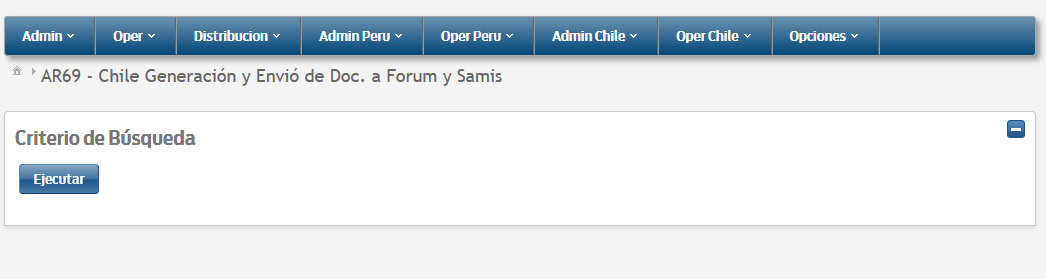
\includegraphics[width=1.00\textwidth]{figuras/image3}
\caption{Pantalla AR69, utilizada para disparar el envío del archivo a Forum por FTP, previo a la integración}\label{fig:2}
\end{figure}

\subsubsection{Gestión de errores y reintentos}

Cuando una entidad bancaria rechaza una solicitud, se presenta una falla de conectividad o se produce un error técnico, VH Connect mantiene el indicador de reporte en estado pendiente, es decir, en \textbf{false}, y genera una notificación hacia Microsoft Teams.

Además, existe un proceso nocturno diario que reintenta el envío de las facturas que no fueron reportadas exitosamente. Este mecanismo permite recuperar operaciones afectadas por errores transitorios sin depender exclusivamente de una intervención manual inmediata.

Antes de efectuar un reintento, la solución deberá verificar si la factura fue reportada exitosamente con anterioridad, con el objetivo de reducir el riesgo de duplicidad en el envío. Los indicadores REPORTED\_FORUM y REPORTED\_SANTANDER permiten identificar las facturas que permanecen pendientes de reporte. Adicionalmente, la tabla 055\_TRANSACCIONES\_CREDITO almacena, para cada unidad, el payload de la última solicitud enviada, la respuesta recibida y el código de estado HTTP en caso de rechazo, lo que permite consultar el detalle técnico del intento más reciente ante un error o una consulta de soporte.

\subsection{Diagrama de arquitectura}

\begin{figure}[H]
\centering
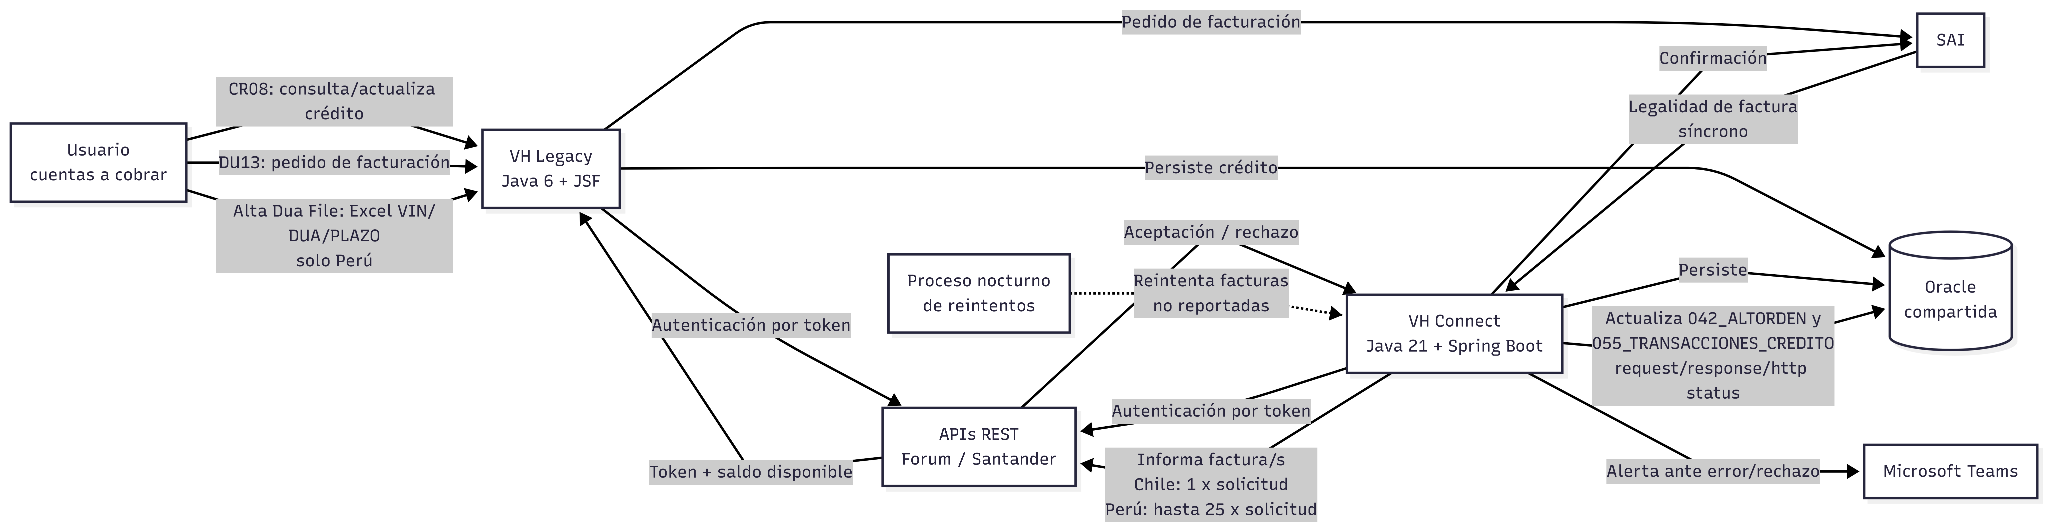
\includegraphics[width=1.00\textwidth]{figuras/image4}
\caption{Diagrama de arquitectura}\label{fig:3}
\end{figure}

La Figura~\ref{fig:3} presenta la arquitectura general de la solución. VH Legacy actúa como punto de entrada para el usuario de cuentas a cobrar, tanto para la consulta y actualización de crédito disponible (autenticándose directamente contra las entidades bancarias) como para la generación de pedidos de facturación y, en el caso de Perú, la carga de datos de DUA y plazo mediante la pantalla Alta Dua File. SAI participa como intermediario, comunicando de forma síncrona a VH Connect la información de las facturas que alcanzan el estado de legalidad. VH Connect centraliza la integración con las entidades bancarias para el envío de facturas, persiste la información en la base de datos Oracle compartida ---incluyendo el resultado de cada operación en la tabla 055\_TRANSACCIONES\_CREDITO--- y notifica por Microsoft Teams ante errores o rechazos. Un proceso nocturno reintenta automáticamente el envío de las facturas que permanecen sin reportar.

\subsection{Justificación de las decisiones arquitectónicas}

La elección de una arquitectura modular, en convivencia con la aplicación legada VH Legacy, responde a la necesidad de garantizar continuidad operativa sin interrumpir los procesos actualmente utilizados por los usuarios de la organización. Reemplazar de forma inmediata un sistema legado implica riesgos operativos significativos ---interrupciones del servicio, curva de aprendizaje para los usuarios, pérdida de funcionalidades no documentadas--- que la organización no está en condiciones de asumir en el corto plazo. Por este motivo, se optó por una estrategia de coexistencia, en la que VH Legacy conserva las funcionalidades de consulta y gestión que los usuarios ya conocen, mientras que la lógica de integración bancaria se traslada a un componente nuevo, VH Connect.

La centralización de la integración bancaria en VH Connect, en lugar de distribuirla entre las aplicaciones existentes, se justifica por razones de mantenibilidad y escalabilidad. Al concentrar en un único componente las reglas de comunicación con cada entidad bancaria ---incluyendo las diferencias de estructura entre Chile y Perú---, se evita duplicar lógica de negocio en distintas aplicaciones y se facilita la incorporación de nuevas entidades bancarias o países en el futuro, sin necesidad de modificar VH Legacy o SAI.

La decisión de utilizar Java 21 con Spring Boot para VH Connect, en contraste con el Java 6 de VH Legacy, responde a la necesidad de contar con un stack tecnológico moderno que facilite el consumo y la exposición de servicios REST, así como la implementación de mecanismos de resiliencia (reintentos, manejo de errores) que la tecnología legada no soporta de manera nativa.

Por su parte, la decisión de mantener una base de datos Oracle compartida entre VH Legacy y VH Connect ---en lugar de introducir una base de datos independiente para el nuevo componente--- prioriza la continuidad operativa y evita la duplicación de información crítica del negocio (concesionarios, casas matrices, facturas). Esta decisión introduce, sin embargo, la necesidad de definir con claridad qué información administra cada aplicación, aspecto que se retoma en la sección de diseño de base de datos.

Finalmente, la comunicación síncrona entre SAI y VH Connect se eligió por sobre un esquema asincrónico debido a que el flujo de negocio requiere una confirmación inmediata de que la legalidad de la factura fue recibida y persistida correctamente, antes de que SAI continúe con los pasos siguientes del proceso de facturación.

\section{Recursos, tecnologías y stack utilizado}

\subsection{Tecnologías de software}

VH Legacy está desarrollada en Java 6, empaquetada en archivos JAR, con una interfaz de usuario implementada mediante JavaServer Faces. VH Connect, por su parte, está desarrollada en Java 21 utilizando el framework Spring Boot, con Gradle como herramienta de construcción y gestión de dependencias. Esta diferencia tecnológica entre ambas aplicaciones refleja la convivencia planteada en la arquitectura de la solución: VH Legacy conserva su stack original para no interrumpir la operatoria existente, mientras que VH Connect incorpora un stack moderno orientado al consumo y la exposición de servicios REST.

\subsection{Infraestructura y entornos}

VH Legacy se ejecuta sobre la plataforma OpenShift. VH Connect, en cambio, se aloja sobre la infraestructura de Google Cloud Platform. Ambas aplicaciones cuentan con ambientes diferenciados de desarrollo (dev), control de calidad (qa) y producción (prod). Las entidades bancarias, en cambio, no ofrecen la misma granularidad de ambientes: para Chile se dispone de ambientes de desarrollo y producción, mientras que, para Perú, la entidad bancaria únicamente expone un ambiente de producción. Esta limitación condiciona las pruebas de integración con la entidad peruana, que deben realizarse directamente contra el ambiente productivo con los recaudos correspondientes.

\subsection{Herramientas de monitoreo y notificación}

La solución no incorpora, en su estado actual, herramientas dedicadas de monitoreo o gestión de logs (como plataformas de observabilidad o dashboards centralizados). El seguimiento operativo se realiza exclusivamente mediante notificaciones enviadas a Microsoft Teams ante errores técnicos, rechazos bancarios o fallas de comunicación. Esta limitación se identifica como una oportunidad de mejora, dado que la ausencia de un historial centralizado de eventos dificulta el análisis retrospectivo de incidentes y la medición de indicadores operativos a lo largo del tiempo.

\section{Diseño de base de datos}

\subsection{Motor de base de datos seleccionado}

El motor de base de datos utilizado por la solución es Oracle, compartido entre VH Legacy y VH Connect. La elección de mantener un único motor y una única base de datos compartida, en lugar de introducir un motor independiente para el nuevo componente, responde a criterios de continuidad operativa: evita duplicar información crítica del negocio (concesionarios, casas matrices, facturas, unidades) que ya es administrada por el sistema legado, y permite que ambas aplicaciones trabajen sobre una única fuente de verdad para los datos compartidos.

\subsection{Modelo de datos y entidades principales}

El modelo de datos, acotado al alcance de este trabajo ---gestión de crédito y datos enviados a la entidad bancaria---, se organiza alrededor de seis tablas principales dentro de la base de datos Oracle compartida: 002\_UNIDADES, 010\_CLIENTES, 222\_MODELOS, 042\_ALTORDEN, 055\_TRANSACCIONES\_CREDITO y 040\_LOTES\_FACT. A lo largo de este documento las tablas se identifican por su número y nombre lógico, aunque físicamente siguen la convención de nombres del sistema legado. Las tablas preexistentes se replican por país, ya que la aplicación opera para Argentina, Chile y Perú: su nombre físico antepone el prefijo TVH seguido del código del país, de modo que la tabla lógica 042\_ALTORDEN corresponde a TVHCH042\_ALTORDEN para Chile y TVHPE042\_ALTORDEN para Perú, ambas con la misma estructura. En cambio, las dos tablas incorporadas por este proyecto, TTVH055\_TRANSACCIONES\_CREDITO y TTVH040\_LOTES\_FACT, son únicas y compartidas por ambos países, y el país de cada registro se identifica mediante la columna DICSUB03\_D309. En todos los casos, las columnas llevan el prefijo TVH seguido del número de la tabla, como en TVH042\_LOTE o TVH055\_REQUEST.

La tabla \textbf{002\_UNIDADES} constituye la entidad central del modelo, dado que concentra la información de cada unidad facturada, incluyendo el VIN, el número de factura y, cuando corresponde, la serie o el punto de venta. A partir de esta tabla se establecen las relaciones con el resto de las entidades del modelo.

La tabla \textbf{010\_CLIENTES} almacena la información de la casa matriz o concesionario, incluyendo su identificación tributaria (RUT para Chile, RUC para Perú), su razón social y los saldos de crédito disponible y facturado. Cada registro de 002\_UNIDADES se asocia a un concesionario de 010\_CLIENTES a través del código de concesionario.

La tabla \textbf{222\_MODELOS} contiene los datos descriptivos de cada modelo de vehículo facturado, tales como la descripción y el peso. Su asociación con 002\_UNIDADES se realiza mediante los datos de catálogo del vehículo (MYVTA, TMA y SEQ), que permiten identificar de manera unívoca el modelo correspondiente a cada unidad.

Finalmente, la tabla 042\_ALTORDEN almacena los indicadores REPORTED\_FORUM y REPORTED\_SANTANDER, que permiten identificar si una unidad fue reportada exitosamente a la entidad bancaria correspondiente. Siguiendo la convención del sistema legado, estos indicadores no se definen como campos booleanos, sino como campos de tipo CHAR de una posición. El campo permanece vacío hasta que la unidad se envía a SAI desde la pantalla DU13; cuando SAI confirma la recepción del pedido de facturación, toma el valor N, que indica que la factura está pendiente de informarse a la entidad bancaria. Esta confirmación es distinta de la notificación de legalidad, que SAI envía más adelante y que dispara el informe al banco; una vez que la entidad acepta la factura, el indicador pasa al valor Y. Su asociación con 002\_UNIDADES se realiza a través del número de factura, lo que permite vincular cada resultado de reporte con la unidad facturada que le dio origen.

Adicionalmente, la tabla \textbf{055\_TRANSACCIONES\_CREDITO} almacena el detalle técnico de cada operación de informe hacia las entidades bancarias, incluyendo el código de país, el payload de la solicitud (request), la respuesta recibida (response) y, en caso de rechazo, el código de estado HTTP correspondiente. Su asociación con 002\_UNIDADES se realiza a través del VIN. Esta tabla se utiliza para ambas entidades bancarias y cada registro se actualiza con la información del intento más reciente.

Para el caso particular de Perú, la tabla incluye además el campo INFO\_ADICIONAL, en formato JSON, donde se almacenan valores como el DUA y el plazo asociado a la unidad. Esta información no se encuentra disponible en ningún otro sistema y es cargada manualmente por el usuario a través de una pantalla de VH Legacy mediante la carga de un archivo Excel con las columnas VIN, DUA y PLAZO, que dispara un proceso encargado de persistir dichos valores en la tabla.

En conjunto, estas relaciones posicionan a 002\_UNIDADES como entidad central del modelo de datos, vinculada a 010\_CLIENTES, 222\_MODELOS, 042\_ALTORDEN y 055\_TRANSACCIONES\_CREDITO.

Adicionalmente, se incorpora la tabla \textbf{040\_LOTES\_FACT}, compuesta por el código de país en formato ISO (por ejemplo, CHL o PER), la fecha de envío del lote, y el número de lote, generado mediante una secuencia que garantiza su unicidad. La tabla 042\_ALTORDEN incorpora, a su vez, el campo \textbf{TVH042\_LOTE}, que almacena el número de lote al que pertenece cada unidad, estableciendo así la relación entre ambas tablas.

\subsection{Integridad, seguridad y trazabilidad}

Dado que la base de datos es compartida entre dos aplicaciones con ciclos de desarrollo independientes, la solución requiere definir con claridad qué información administra cada componente, con el fin de preservar la integridad de los datos y evitar inconsistencias derivadas de modificaciones concurrentes o mal delimitadas.

La trazabilidad de las operaciones se sostiene sobre los indicadores REPORTED\_FORUM y REPORTED\_SANTANDER (con valores Y/N), complementados por la tabla 055\_TRANSACCIONES\_CREDITO, que registra el detalle técnico del intento más reciente de cada operación. El funcionamiento de este mecanismo, junto con sus limitaciones y mejoras futuras identificadas, se desarrolla en profundidad en la sección ``Trazabilidad, auditoría y gestión de errores''.

\section{Diseño de interfaz y experiencia de usuario}

\subsection{Usuarios de la solución}

Los usuarios directos de la solución, en el flujo abordado por este trabajo, pertenecen al área de cuentas a cobrar, responsable de la gestión de crédito y de la facturación de las unidades. Este equipo interactúa con la solución exclusivamente a través de VH Legacy, dado que VH Connect no expone una interfaz de usuario propia.

\subsection{Pantallas y funcionalidades principales}

El flujo de trabajo del usuario se apoya en las pantallas existentes de VH Legacy. Las pantallas CR08 y CR12 permiten verificar y actualizar el crédito disponible de cada concesionario, información que resulta necesaria antes de autorizar la facturación de una unidad. La pantalla DU13, por su parte, concentra la funcionalidad de facturación, desde donde el usuario genera el pedido que da inicio al flujo automatizado hacia SAI y, posteriormente, hacia VH Connect.

\begin{figure}[H]
\centering
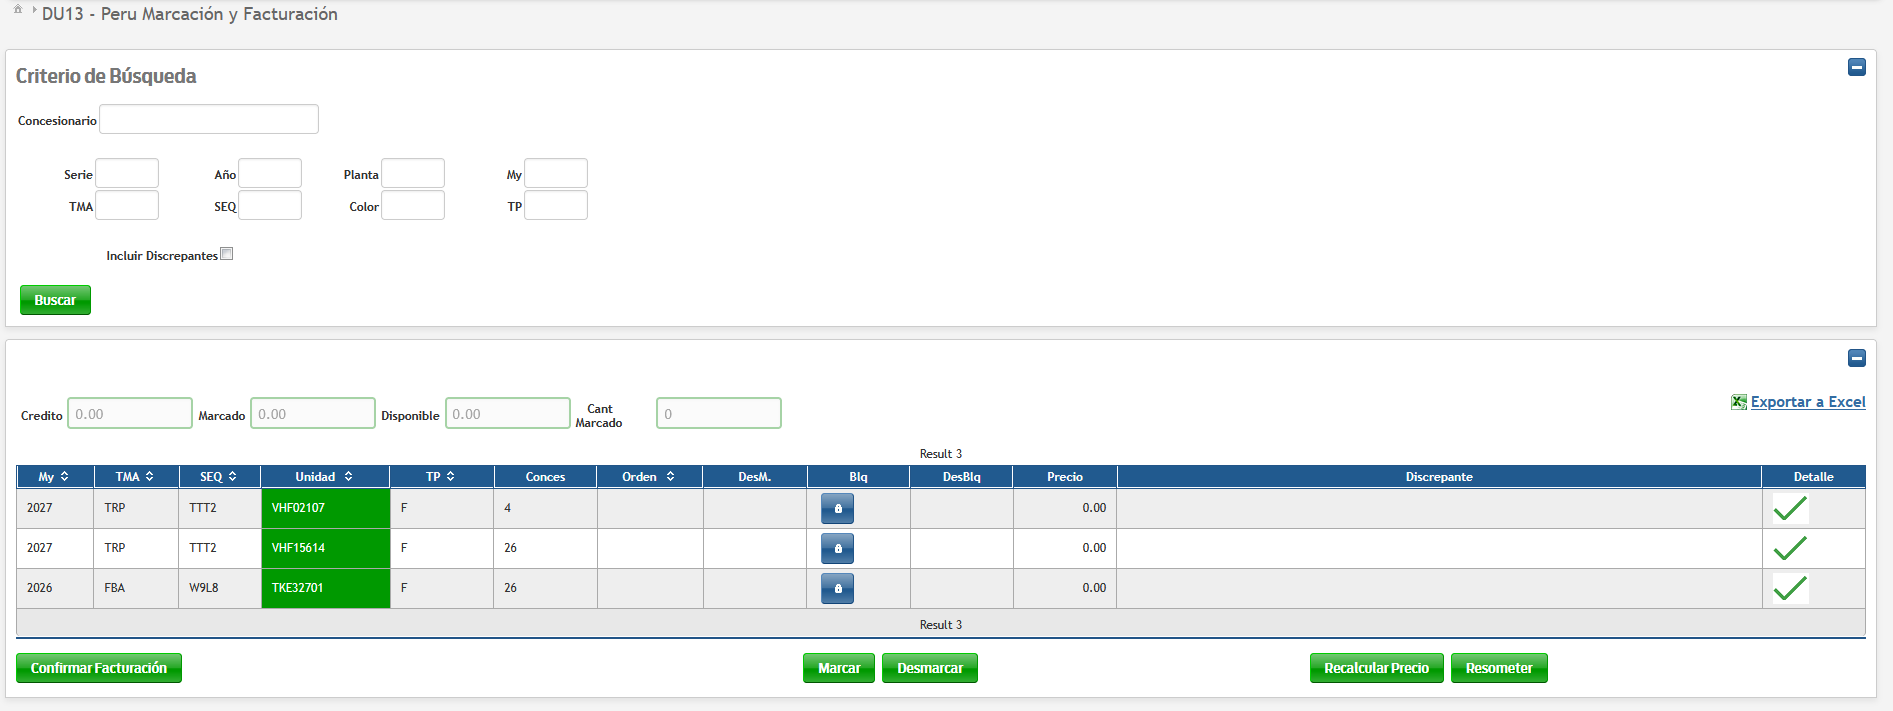
\includegraphics[width=1.00\textwidth]{figuras/image5}
\caption{DU13 Perú}\label{fig:4}
\end{figure}

\begin{figure}[H]
\centering
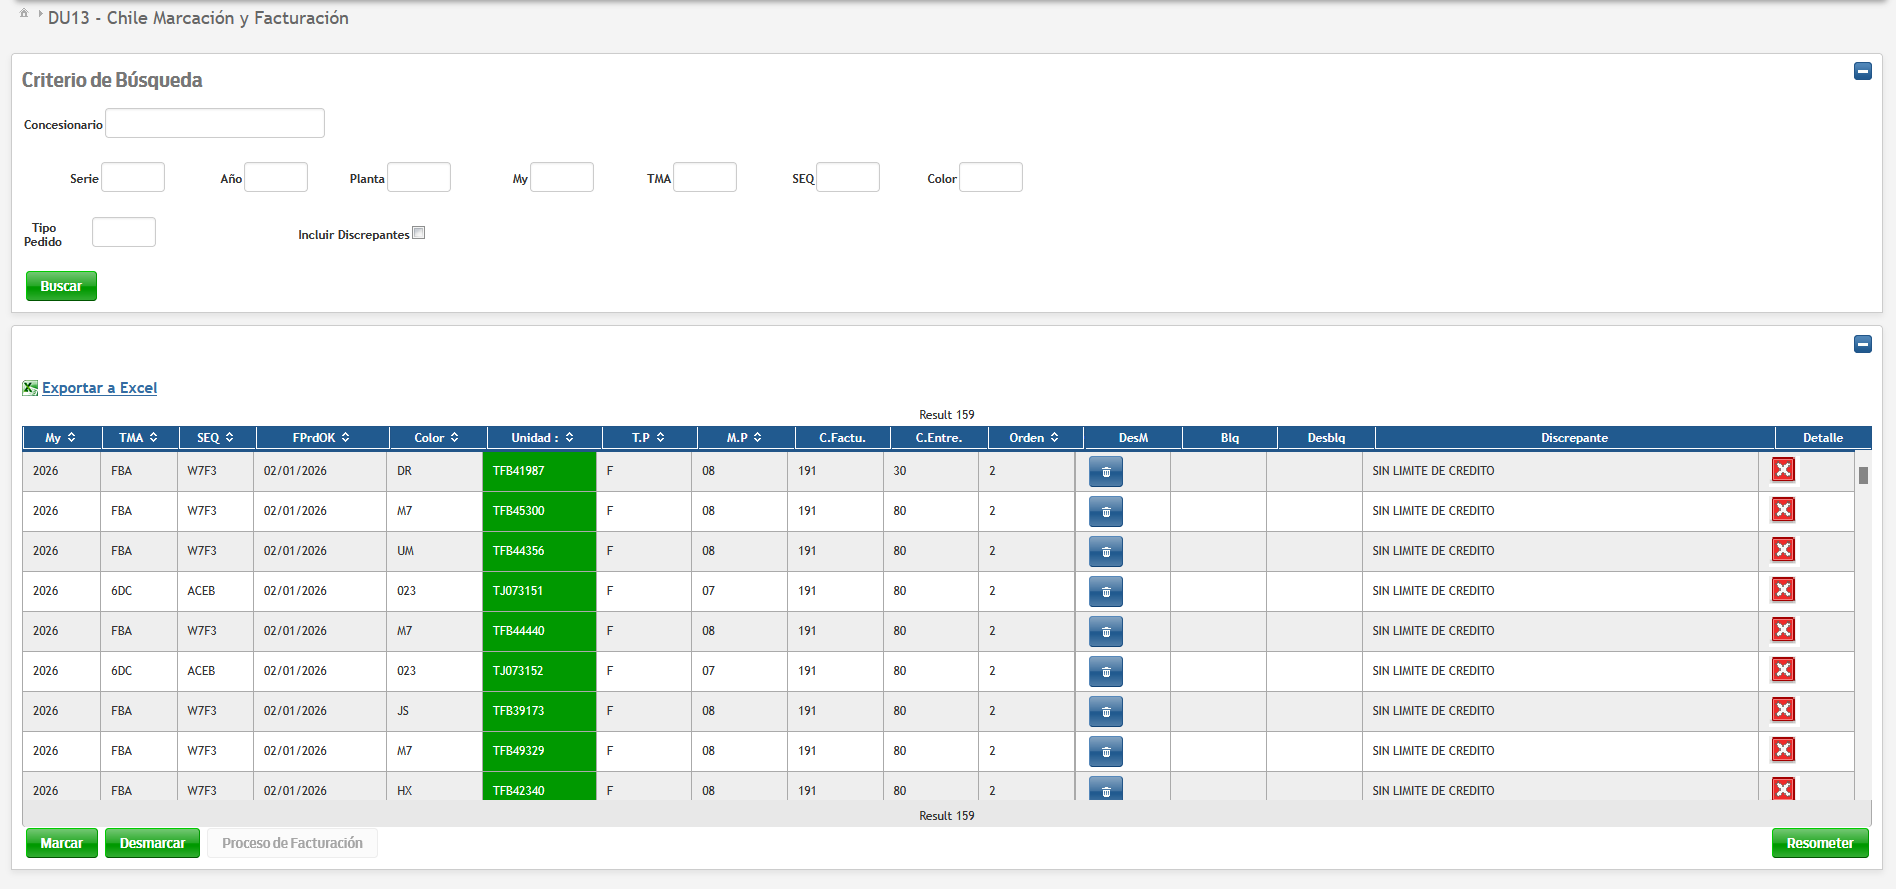
\includegraphics[width=1.00\textwidth]{figuras/image6}
\caption{DU13 Chile}\label{fig:5}
\end{figure}

VH Connect no incorpora interfaz de usuario: su función se limita a la integración backend con las entidades bancarias, por lo que no forma parte de la experiencia de usuario directa, sino que opera de manera transparente para el equipo de cuentas a cobrar.

Adicionalmente, para el caso de Perú, VH Legacy incorpora la pantalla \textbf{Alta Dua File}, mediante la cual el usuario carga un archivo Excel con las columnas VIN, DUA y PLAZO. El procesamiento de este archivo se ejecuta de forma batch, permitiendo al usuario continuar operando en otras pantallas mientras el proceso se completa. Al finalizar, el usuario recibe una notificación por correo electrónico indicando el resultado de la carga; en caso de que algún registro no haya podido procesarse correctamente, el correo detalla los datos afectados.

\subsection{Decisión de diseño, usabilidad y accesibilidad}

El nuevo diseño introduce una unificación de pantallas orientada a simplificar la experiencia del usuario, aplicable específicamente al caso de Chile. Previamente, la consulta de crédito disponible se encontraba dividida entre dos pantallas: CR08, que mostraba el saldo correspondiente a unidades pesadas (vehículos utilitarios), y CR12, que mostraba el saldo correspondiente a unidades livianas (el resto de los modelos). Esta separación obligaba al usuario de cuentas a cobrar a consultar dos pantallas distintas según el tipo de unidad involucrada, incrementando la cantidad de pasos necesarios para verificar el crédito disponible de un concesionario.

\begin{figure}[H]
\centering
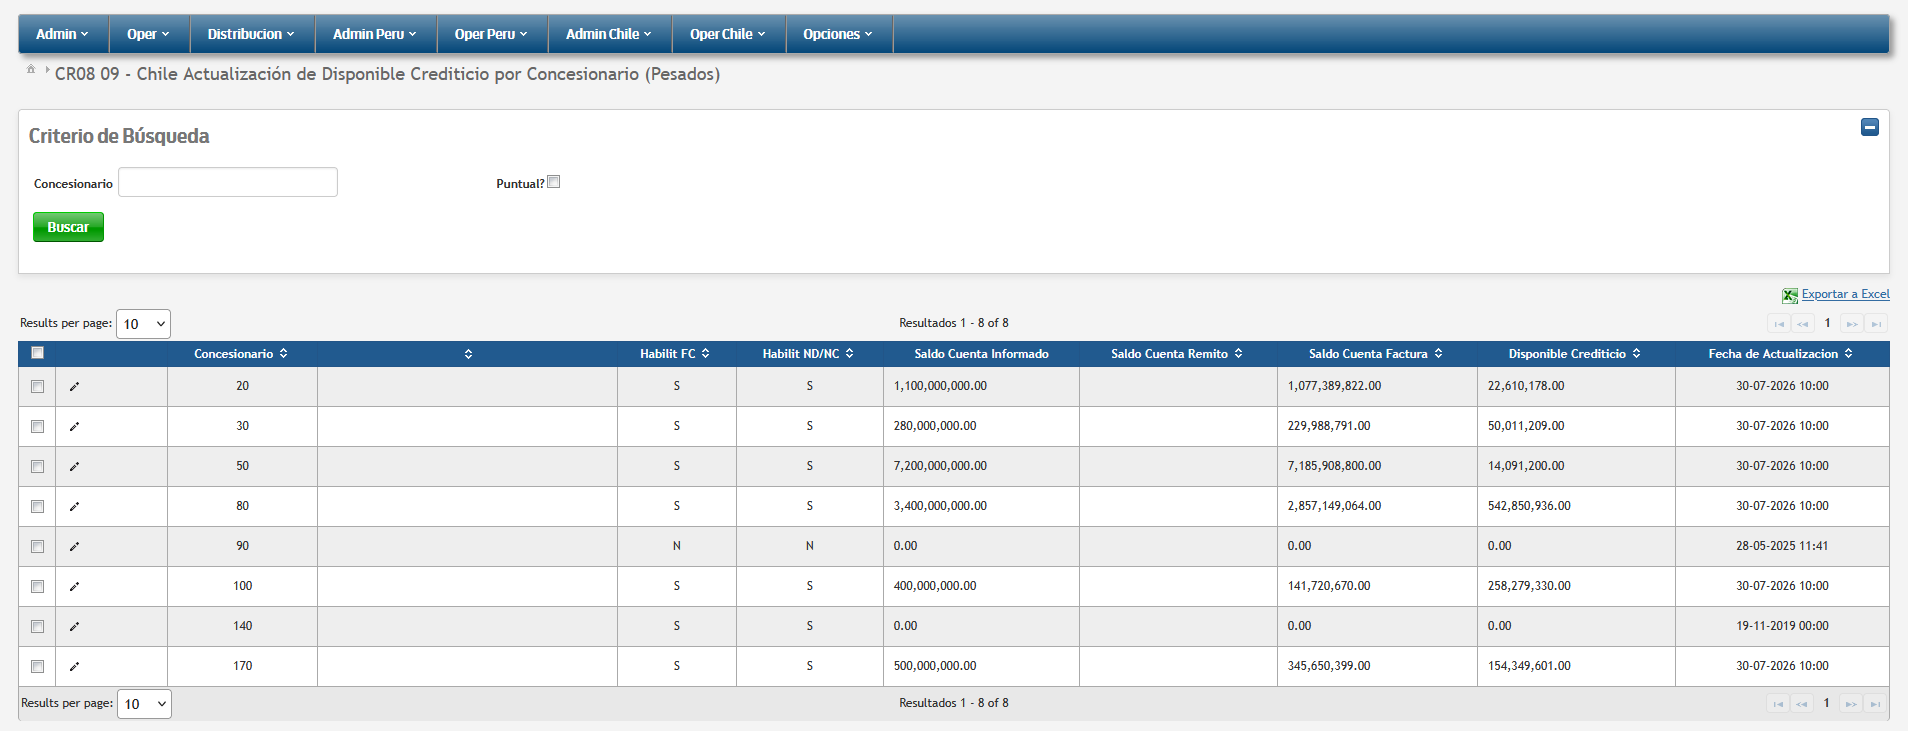
\includegraphics[width=1.00\textwidth]{figuras/image7}
\caption{Pantalla CR08 (Chile) --- consulta de disponible crediticio de unidades pesadas, previo a la unificación}\label{fig:6}
\end{figure}

\begin{figure}[H]
\centering
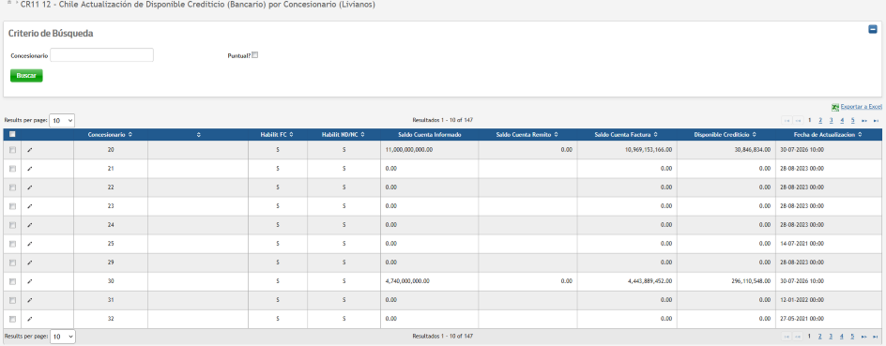
\includegraphics[width=1.00\textwidth]{figuras/image8}
\caption{Pantalla CR12 (Chile) --- consulta de disponible crediticio de unidades livianas, previo a la unificación}\label{fig:7}
\end{figure}

El diseño propuesto unifica ambas consultas en la pantalla CR08, incorporando una separación clara dentro de la misma pantalla entre el saldo disponible y facturado correspondiente a unidades livianas, y el saldo disponible y facturado correspondiente a unidades pesadas. Esta decisión reduce la cantidad de pantallas que el usuario debe consultar para obtener una visión completa del crédito de un concesionario, mejorando la eficiencia operativa sin requerir que el usuario aprenda una interfaz nueva, dado que se apoya sobre una pantalla ya conocida. Cabe aclarar que esta distinción entre unidades livianas y pesadas es propia de Chile: en Perú, el sistema no maneja dicha categorización, por lo que la pantalla equivalente (CR08) no requiere esta separación.

\begin{figure}[H]
\centering
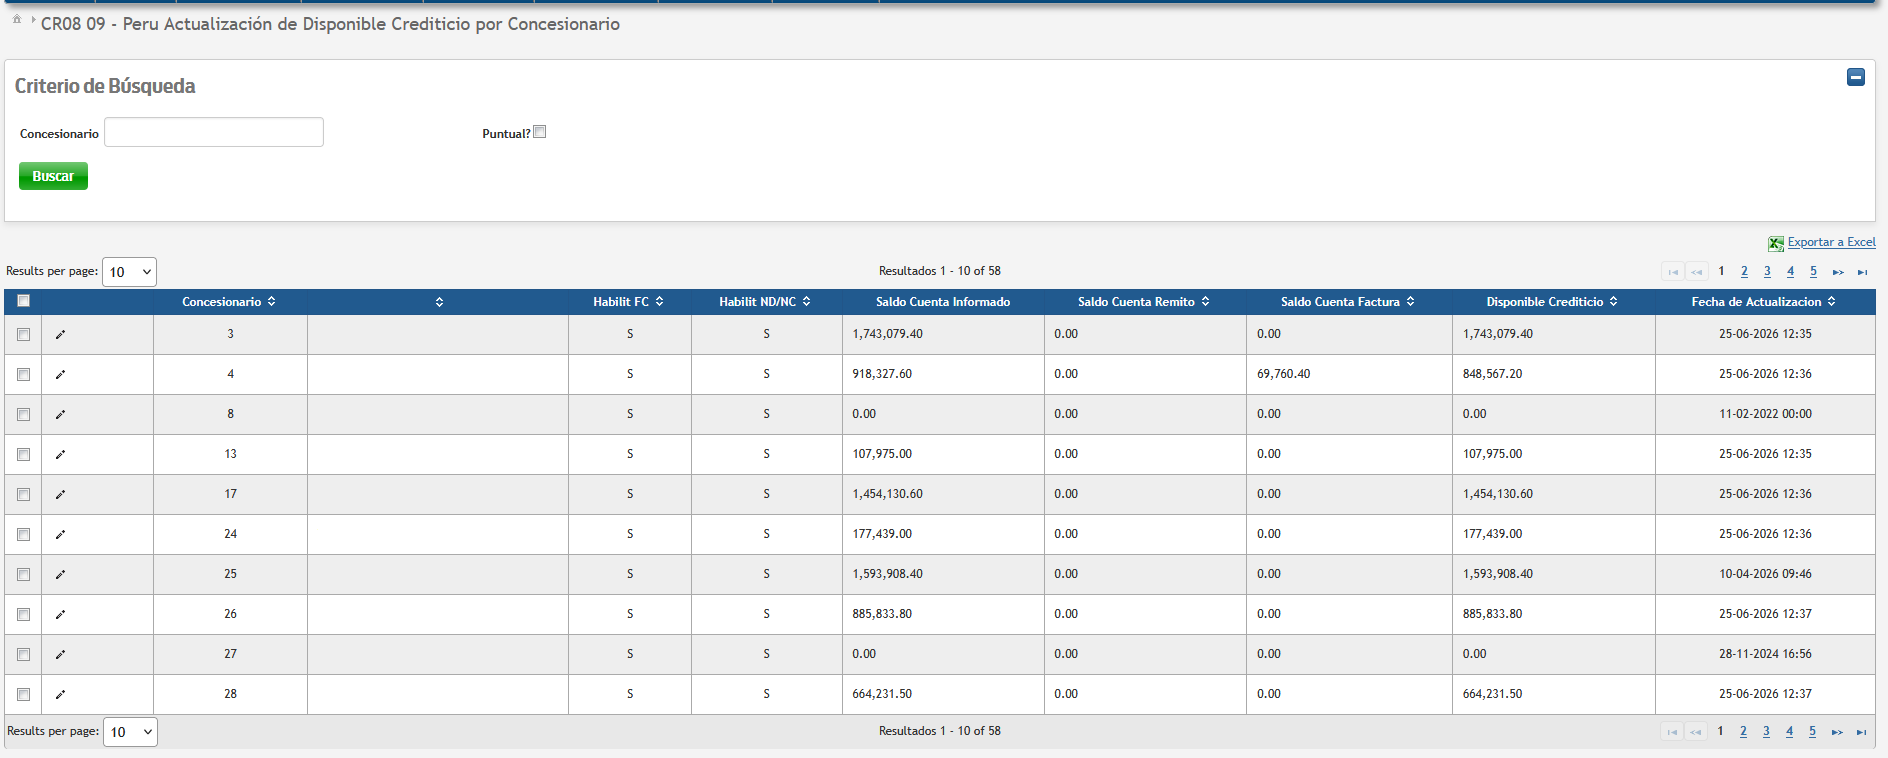
\includegraphics[width=1.00\textwidth]{figuras/image9}
\caption{CR08 Perú}\label{fig:8}
\end{figure}

Esta carencia de automatismo para distinguir entre unidades livianas y pesadas añade complejidad operativa al proceso actual, reforzando la necesidad de unificar ambas consultas en una única pantalla.

\subsection{Validación de diseño}

La decisión de unificar CR08 y CR12 surgió a partir de una devolución informal del equipo de cuentas a cobrar, obtenida en una conversación presencial durante el relevamiento de la solución. Si bien no se trató de una instancia formal de validación de usabilidad (como una prueba estructurada con usuarios), el comentario reflejó una dificultad concreta percibida por los usuarios en su operatoria diaria ---la necesidad de consultar dos pantallas distintas según el tipo de unidad--- y motivó directamente la decisión de diseño adoptada. Se identifica como mejora futura la incorporación de instancias más formales de validación de usabilidad antes de definir cambios de interfaz, de manera de sustentar estas decisiones con evidencia más sistemática.

\section{Seguridad, calidad y control de versiones}

\subsection{Autenticación y autorización}

La autenticación contra las entidades bancarias se resuelve mediante un esquema de token, propio de cada entidad, y es utilizada tanto por VH Legacy como por VH Connect: VH Legacy se autentica para consultar y actualizar las líneas de crédito, mientras que VH Connect lo hace para informar las facturas a la entidad bancaria. Ambos componentes utilizan el mismo endpoint y los mismos parámetros de autenticación de cada entidad; la implementación varía únicamente por la diferencia tecnológica entre ambas aplicaciones (Java 6 en VH Legacy, Java 21 en VH Connect).

Previo a realizar una operación contra la entidad bancaria correspondiente, cada aplicación debe autenticarse contra el endpoint específico expuesto por dicha entidad, el cual retorna un token que se utiliza en las solicitudes subsiguientes.

La estructura de la solicitud de autenticación varía según la entidad. En el caso de Santander, la autenticación se realiza mediante una solicitud cuyo cuerpo (body) contiene las credenciales en formato JSON, incluyendo usuario y contraseña. En el caso de Forum, en cambio, los parámetros de autenticación se envían a través del header de la solicitud. En ambos casos, la respuesta exitosa retorna un token que debe incluirse en las llamadas posteriores a la API correspondiente.

Esta heterogeneidad en los mecanismos de autenticación entre entidades bancarias refuerza la necesidad de que cada aplicación conozca las particularidades de cada integración bancaria con la que interactúa.

\subsection{Gestión de credenciales bancarias}

La gestión de credenciales difiere según la aplicación. En VH Connect, las credenciales de acceso a las entidades bancarias se almacenan en Secret Manager de Google Cloud Platform, evitando que dicha información sensible resida en el código fuente, en archivos de configuración o en la base de datos de la aplicación. En VH Legacy, dichas credenciales se gestionan dentro de la plataforma OpenShift sobre la cual se despliega la aplicación, de manera independiente del esquema utilizado por VH Connect.

En ambos casos, los tokens de autenticación obtenidos se mantienen en memoria durante la ejecución de la aplicación correspondiente. Ante un reinicio, cada aplicación valida si existe un token previamente obtenido y, en caso afirmativo, verifica su vigencia; si el token no existe o se encuentra vencido, se genera uno nuevo a partir de las credenciales almacenadas. Este mecanismo evita solicitar un nuevo token en cada llamada a la API bancaria, reduciendo la cantidad de autenticaciones innecesarias contra las entidades financieras.

En cuanto a la rotación de credenciales, la solución no cuenta con un mecanismo propio y automatizado para tal fin, tanto en VH Legacy como en VH Connect. Ante la necesidad de modificar una credencial, la actualización es iniciada por la propia entidad bancaria, que notifica dicho requerimiento al equipo responsable. Esta dependencia de un proceso externo y manual se identifica como una limitación de la solución actual, y se propone como mejora futura la incorporación de un mecanismo de rotación periódica y automatizada de credenciales para ambas aplicaciones.

\subsection{Trazabilidad, auditoría y gestión de errores}

La trazabilidad de las operaciones se sostiene sobre los indicadores REPORTED\_FORUM y REPORTED\_SANTANDER (con valores Y/N), que permiten identificar en todo momento si una factura fue reportada exitosamente a cada entidad bancaria, complementados por la tabla 055\_TRANSACCIONES\_CREDITO, que almacena el payload de la solicitud, la respuesta de la entidad bancaria y, ante un rechazo, el código de estado HTTP del intento más reciente por unidad.

Dado que los registros de \textbf{055\_TRANSACCIONES\_CREDITO} se actualizan en cada intento en lugar de generar un nuevo registro histórico, la solución permite inspeccionar el detalle técnico del último intento, pero no conserva un historial completo de todos los intentos previos. Se identifica como mejora futura convertir este mecanismo en un esquema de inserción (append-only), que permita reconstruir la secuencia completa de eventos de cada operación ante una auditoría o un incidente.

\subsection{Estrategia de pruebas}

La estrategia de pruebas se concentra en VH Connect, componente sobre el cual se implementan pruebas unitarias mediante JUnit. VH Legacy, por tratarse de una aplicación legada, no cuenta con una suite de pruebas automatizadas, lo cual constituye una limitación reconocida del proyecto y un riesgo a considerar ante futuras modificaciones sobre dicho componente.

\subsection{Control de versiones}

El control de versiones de las aplicaciones se gestiona mediante GitHub, siguiendo un flujo de ramas alineado con los ambientes de la solución (dev, qa y prod). Ante el desarrollo de una nueva funcionalidad, se crea una rama a partir de dev, sobre la cual se realiza el trabajo correspondiente. Una vez finalizado el desarrollo, se genera un pull request hacia dev; superada esta instancia, los cambios se promueven de dev a qa y, finalmente, de qa a prod. Este esquema permite validar los cambios en ambientes intermedios antes de su llegada a producción, y sostiene el proceso de integración y despliegue continuo descrito en la sección correspondiente.

\section{Alcance del prototipo o MVP}

El alcance del prototipo (MVP) contempla la implementación completa del flujo de facturación automatizada para ambos países considerados en este trabajo, Chile y Perú, incluyendo la consulta y actualización de crédito disponible, la recepción de legalidades de factura desde SAI, el envío de facturas a la entidad bancaria correspondiente y la gestión de errores y reintentos. Quedan fuera del alcance del MVP la incorporación de nuevas entidades bancarias adicionales a Forum y Santander, la extensión a otros países como Argentina, y la incorporación de herramientas de monitoreo u observabilidad dedicadas, aspectos que se identifican como líneas de trabajo futuras.

Asimismo, el alcance del MVP contempla la gestión de lotes de facturación, incluyendo la notificación automática por correo electrónico ante la finalización de un lote y el disparo del informe de facturas hacia la entidad bancaria correspondiente una vez completado dicho lote.

\section{Síntesis del capítulo}

A lo largo de este capítulo se presentó la justificación técnica y el diseño de la solución propuesta para automatizar el proceso de facturación de unidades financiadas y su comunicación con las entidades bancarias de Chile y Perú.

Se optó por una arquitectura modular que prioriza la continuidad operativa, permitiendo la convivencia entre la aplicación legada VH Legacy y el nuevo componente VH Connect, encargado de centralizar la integración con las entidades bancarias. Esta decisión evita interrumpir la operatoria de los usuarios del área de cuentas a cobrar, quienes continúan trabajando sobre pantallas ya conocidas (CR08, CR12 y DU13), a la vez que incorpora un stack tecnológico moderno ---Java 21 con Spring Boot--- orientado al consumo y exposición de servicios REST.

En cuanto al modelo de datos, se definió un conjunto acotado de tablas dentro de la base de datos Oracle compartida (010\_CLIENTES, 002\_UNIDADES, 222\_MODELOS, 042\_ALTORDEN, 055\_TRANSACCIONES\_CREDITO y 040\_LOTES\_FACT), centradas específicamente en la información necesaria para la gestión de crédito y la comunicación con los bancos, con 002\_UNIDADES como entidad central del modelo. La tabla 055\_TRANSACCIONES\_CREDITO, en particular, mejora la trazabilidad al registrar el payload y la respuesta de cada operación bancaria, y sostiene además la carga de datos específicos de Perú (DUA y plazo) a través de la nueva pantalla Alta Dua File.

Desde el punto de vista de la experiencia de usuario, se destacó la unificación de las pantallas CR08 y CR12 en una única pantalla que separa el crédito de unidades livianas y pesadas, decisión motivada por una devolución informal del propio equipo de cuentas a cobrar, lo que evidencia una oportunidad de mejora futura en cuanto a instancias más formales de validación de usabilidad.

En materia de seguridad, se definió un esquema de autenticación por token propio de cada entidad bancaria, utilizado tanto por VH Legacy como por VH Connect, con almacenamiento de credenciales en Secret Manager de Google Cloud Platform para VH Connect y en la plataforma OpenShift para VH Legacy, junto con un mecanismo de gestión de tokens en memoria.

Finalmente, se describió el esquema de control de versiones y despliegue continuo, basado en GitHub y en la promoción de cambios a través de los ambientes dev, qa y prod, delimitando explícitamente que las decisiones de infraestructura subyacente exceden el alcance de este trabajo, cuyo foco central es la lógica de negocio asociada a la actualización y comunicación del saldo de crédito con las entidades bancarias.
